\chapter{Blockchain 1.0 - Wie Bitcoin funktioniert}
Mit Fortschritt im Bereich Kryptographie begann auch das Interesse von Forschern an digitalen Währungen. 
Das Problem dieser frühen Projekte bestand jedoch darin, dass sie einen sogenannten \emph{Central Point of Failure}, also eine zentralisierte Schwachstelle besaßen. 
Beispielsweise könnten die Konten von Nutzern zwar kryptografisch gesichert, jedoch von zentralen Stellen wie Banken verwaltet werden müssen.
Ein wichtiges Problem, welches es mithilfe eines neuartigen Geldsystems zu lösen gilt, ist das sogenannte \emph{Double Spending Problem}. Es muss durch gewisse Mechanismen verhindert werden, dass bösartige Akteure die selben Geldwerte für mehrere Transaktionen verwenden. Bei physischem Geld, also Geldscheinen, Münzen, etc. verhindern komplexe Drucktechniken die Verbreitung von Falschgeld und dadurch dass ein Geldschein nur einmal existieren kann, ist dieser nur für eine Transaktion zu verwenden.
Versucht man nun diese Geldwerte gänzlich digital zu verwalten, so liegt die Verantwortung für eine korrekte Beobachtung und Verwaltung bei einer zentralen Stelle wie einer Bank. Diese könnte als Angriffsstelle für Antagonisten dienen und stellt somit eine Gefahr für das System dar.
Dieses Kapitel beschäftigt sich mit der traditionellen Funktionsweise von Geld und wie mithilfe eines dezentralen Systems ein zentraler Fehlerpunkt vermieden werden kann. 
\section{Funktionsweise von Geld}
\cite{mankiw_taylor_2018} bezeichnen Geld als ein Bündel von Aktiva, das die Menschen in einer Volkswirtschaft regemäßig dazu verwenden, Waren und Dienstleistungen von anderen Menschen zu erwerben.
Es erlaubt den Parteien einem Tauschgeschäft, bei dem beide Seiten mit dem Gut des Tauschpartners zufrieden sein müssen, zu entgehen und ermöglicht stattdessen eine effiziente Allokation von Ressourcen. Zugleich stellt Geld sicher, dass das eigene Kapital den Wert auch in Zukunft behält.
Damit ein Handelsgut als Geld angesehen werden kann, muss es drei Funktionen erfüllen können.
Fundamental ist, dass das Handelsgut generell als Tausch- bzw. Zahlungsmittel akzeptiert wird. Theoretisch könnte man versuchen, sein Abendessen mit dem eigenen Fahrrad zu bezahlen, doch kommt man in der Praxis mit dieser Strategie nicht weit.
Des Weiteren muss das Tauschgeschäft als Recheneinheit fungieren können. Dies ist notwendig, da anhand dessen die relativen Preise anderer Waren in der Marktwirtschaft ermittelt werden müssen.
Zuletzt muss sichergestellt sein, dass das Handelsgut wie bereits erwähnt in Zukunft auch seine Kaufkraft behält. Jemand, der es als Zahlungsmittel akzeptiert, muss sich darauf verlassen können, dass es auch für zukünftige Geschäfte verwendet werden kann.\\

Bei den Geldformen unterscheidet man zwischen Warengeld und Rechengeld. Diese unterscheiden sich in ihrem intrinsischen Wert, also darin, ob sie auch außerhalb von Tauschgeschäften einen Nutzen finden. Ein Beispiel für Warengeld ist Gold, welches neben Tauschgeschäften auch industriell verarbeitet werden kann.
Papiergeld hingegen bietet abseits des Tauschgeschäftes keinen Nutzen für den Besitzer. Um trotzdem den Wert des Geldes gewährleisten zu können, wird es von Seiten des Staats als universelles Zahlungsmittel in der jeweiligen Marktwirtschaft bestimmt.\\

Eine weitere wichtige Rolle im Finanzsystem nehmen Zentralbanken ein. Sie überwachen das Bankensystem und steuern über eine geeignete Geldpolitik das Geldangebot auf dem Markt.
Durch das Drucken von Geld und den anschließenden Kauf von Wertpapieren können sie das Geldangebot erhöhen. Um es wiederum zu verringern, verkaufen sie Wertpapiere und nehmen das erhaltene Geld aus dem Umlauf.\\

Eine Währung, die zum Verwalten und Versenden von monetärem Wert dient, hat drei technische Anforderungen zu erfüllen:
\begin{enumerate}
	\item Sicherstellung des Wertes, also die Authentizität
	\item Garantie dafür, dass die selbe Währung nicht mehr als einmal verwendet werden kann (Double Spending)
	\item Zugang zur Währung nur für befugten Besitzer
\end{enumerate}
TODO
\section{Vorzüge der Blockchain-Technologie}
\section{Theorie der Blockchain-Technologie am Beispiel von Bitcoin}
Auch wenn es andere Projekte für dezentrale Währungen wie B-Money [\cite{dai_1998}] und Hashcash [\cite{back_2002}] gab, begann der Aufschwung digitaler Währungen im Jahr 2008 mit der Veröffentlichung des Bitcoin-Whitepapers  [\cite{nakamoto_whitepaper_2008}]. Diese Publikation trägt den Titel \emph{Bitcoin: A Peer to peer Electronic Cash System}, wurde von einer bis heute unbekannten Person, unter dem Namen \emph{Satoshi Nakamoto} veröffentlicht und kombinierte Technologien ihrer Vorgänger. Statt einer zentralen Verwaltungsstelle handelt es sich bei Bitcoin um ein dezentrales Peer-to-peer Netzwerk zwischen den Nutzern des Bitcoin-Protokolls. Außerdem werden Vermögenswerte nicht durch klassische Münzen auf einem Konto repräsentiert, sondern durch vergangene Transaktionen in einem dezentralen und öffentlichen Transaktionsbuch, dem sogenannten \emph{Ledger}, impliziert. Aufgrund dieser Eigenschaften besteht keine zentrale Angriffsfläche für bösartige Akteure und jeder Akteur im Netzwerk hat Kenntnis über alle Transaktionen. Die folgenden Untersektionen beschäftigen sich mit der Verwaltung und dem Zugang für Nutzer, die Funktionsweise von Transaktionen sowie die Art und Weise, wie die verschiedenen Akteure im Netzwerk zu einem gemeinsamen Konsens kommen.
\subsection{Keys und Adressen}
Als Kryptographie bezeichnet man Verfahren zur Verschlüsselung von Informationen, die schon von den Nazis im zweiten Weltkrieg genutzt wurden [\cite{landwehr_2008}: 19]. 
Mithilfe von Maschinen, den sogenannten \emph{ENIGMA}, verschlüsselten sie wichtige strategische Informationen wie die Aufenthaltsorte von Truppen oder taktische Befehle, die anschließend per Funk überbracht wurden.
Kryptographische Verfahren folgten zu der Zeit dem Prinzip \emph{Security by Obscurity}, nach dem die Sicherheit eines Verschlüsselungsverfahrens davon abhängig ist, ob die Funktionsweise dieser bekannt ist. 
Dies hatte zur Folge, dass im Falle der Nazis, deren ENIGMA-Code durch die Anstrengungen polnischer und später englischer Wissenschaftler um Alan Turing unschädlich gemacht werden konnte [\cite{landwehr_2008}: 18/19].\\

Im Jahr 1976 stellten \emph{Diffie} und \emph{Hellman} die bis dahin unbekannte asymmetrische Verschlüsselung vor, bei der jede Partei ein Schlüsselpaar, bestehend aus privatem und öffentlichem Schlüssel, besitzt [vgl. \cite{diffie_hellman_1976}]. 
Derartige Verfahren sind heutzutage der Standard und werden auch im Bitcoin-System verwendet. Das restliche, sowie folgende Kapitel beziehen sich auf \cite{antanopoulos_2014} und ziehen, wo es nötig ist, zusätzliche Quellen hinzu.\\

Für Bitcoin wird ein Paar aus Schlüsseln erzeugt. 
Dieses Paar besteht aus dem privaten Schlüssel (Private Key), welcher nur dem Besitzer bekannt ist und zum Signieren von Transaktionen nötig ist.
Aus diesem wird durch die Verwendung von Hashing-Verfahren ein öffentlicher Schlüssel (Public key) abgeleitet, mit dem Bitcoins empfangen werden können.
Außerdem kann aufgrund der mathematischen Abhängigkeit zwischen den Schlüsseln eine durch den privaten Schlüssel signierte Transaktion mithilfe des öffentlichen Schlüssels verifiziert werden. Dies geschieht, indem der Absender die Transaktion mit seinem privaten Schlüssel signiert und die Authentizität der Signatur mithilfe des öffentlichen Schlüssels von anderen Akteuren des Netzwerks verifiziert wird. Um Begünstigter einer Transaktion zu sein, muss man eine Adresse besitzen und diese an andere Nutzer des Netzwerks propagieren. Um jene zu erzeugen, wird der öffentliche Schlüssel genutzt, welchen man nicht wieder aus der Adresse rekonstruieren kann. Dies wird in Abbildung 2.1 deutlich:
\begin{figure}[htpb]
	\centering
	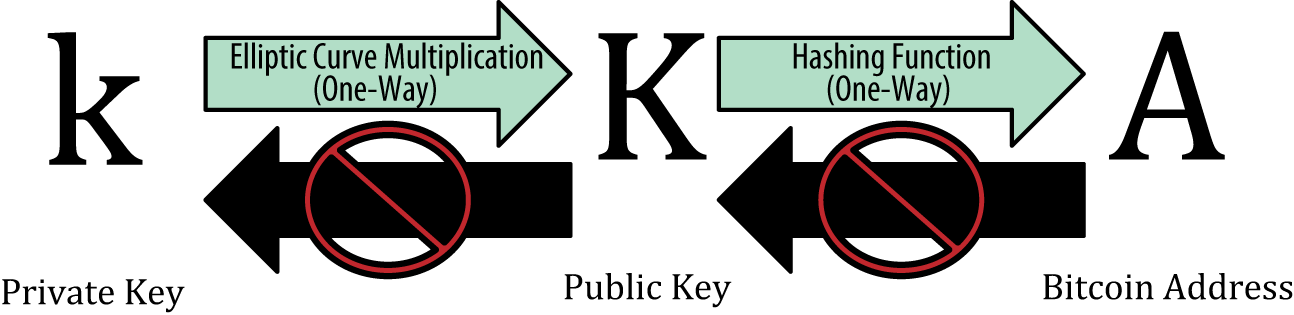
\includegraphics[width=\textwidth]{images/public_and_private_key.png}
	\caption{Generierung der Schlüssel bzw. Adressen aus dem jeweiligen Vorgänger. 
	Quelle: \cite[57]{antanopoulos_2014}}
	\label{6braun:fig:keys}
\end{figure}
\subsubsection{Private Keys}
Ein privater Schlüssel besteht aus einer Zahl von 256 zufälligen Bits. Er wird zum Signieren von Transaktionen und für den Zugriff auf ein Guthaben benötigt. Ohne privaten Schlüssel verliert man als Besitzer von Bitcoin auch den Zugriff auf das eigene Guthaben.\\
Um einen privaten Schlüssel generieren zu können, benötigt man eine sichere Quelle für Zufälligkeit. In anderen Worten: Die Wahl der zufälligen Zahl darf nicht vorhersehbar sein. Dazu verwendet die Bitcoin-Software den Random Number Generator des verwendeten Betriebssystems, kombiniert mit einem menschlichen Input, wie dem Bewegen der Maus [vgl. \cite{antanopoulos_2014}: 58]. Mithilfe des Generators erzeugt man einen zufälligen String, welcher \emph{mehr} als 256 Bits hat. Diesen lässt man anschließend durch den SHA256 Hash-Algorithmus laufen und prüft, ob die resultierende Zahl kleiner ist, als die vom Bitcoin-Protokol gewählte Konstante \emph{n} ($n = 1.1578 * 10^{77}$). Diese Zahl entspricht nach der Ordnung der Gruppe, die in der dort verwendeten elliptischen Kurve entspricht. Nach [\cite{corbellini_2015}] befinden sich alle Punkte der Kurve in dieser Gruppe, weshalb der gewählte private Schlüssel, welcher für die anschließende Generierung eines öffentlichen Schlüssels genutzt wird, nicht außerhalb dieses Bereichs liegen darf.

\subsubsection{Public Keys}
Um einen öffentlichen Schlüssel aus dem privaten generieren zu können, benötigt man ein kryptografisches Verfahren, welches eine Rekonstruktion des Privaten aus dem öffentlichen Schlüssel nicht zulässt.
Das vom Bitcoin-Protokol verwendete Verfahren wird \emph{Elliptic Curve Cryptography} gennant und bedient sich an den Eigenschaften einer Ellipse. Die im Bitcoin-Protokoll verwendete Ellipse trägt den Namen \emph{secp256k1} und hat die, in Abbildung 2.2 vorgestellte, Form:
\begin{figure}[htpb]
	\centering
	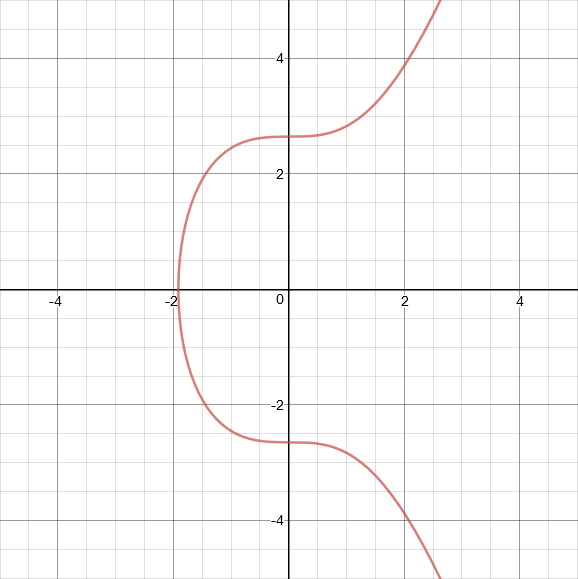
\includegraphics[width=0.7\textwidth]{images/elliptic_graph_cryptography.png}
	\caption{Die von Bitcoin verwendete Ellipse mit der Funktion $y^{2} = x^{3} + 7$ \\TODO: Bessere Grafik}
	\label{6braun:fig:ellipse}
\end{figure}
Um einen öffentlichen Schlüssel zu generieren, wählt man einen Punkt, den sogenannten Generatorpunkt, auf der Ellipse und multipliziert diesen mit dem vorher generierten privaten Schlüssel. Eine Multiplikation kann auch als Addition einer Zahl mit derselben betrachtet werden. Um den Punkt G auf der Ellipse mit sich selbst zu addieren, zieht man an diesem die Tangente und berechnet den Schnittpunkt von Ellipse und der gezogenen Tangente. Anschließend spiegelt man den Punkt an der x-Achse und erhält somit 2G. Diese Addition führt man so oft aus, wie der 256 Bit lange private Schlüssel groß ist, sodass man am Ende einen Punkt (x,y) erhält, welcher als öffentlicher Schlüssel genutzt werden kann. Diesen generierten Schlüssel kann man veröffentlichen, denn aus ihm lässt sich nicht schließen, mit welchem Faktor der Generatorpunkt multipliziert wurde.

\subsubsection{Bitcoin Adressen}
Eine Adresse ist ein aus dem öffentlichen Schlüssel generierter String aus Buchstaben und Zahlen, der den Besitzer des Schlüssels zu einem potentiellen Empfänger einer Transaktion macht. Beim diesem muss es sich allerdings nicht zwangsläufig um eine Person handeln, denn auch Organisationen, geschriebene Skripte, etc. kommen als \emph{abstrakter} Empfänger in Frage.
So wie der öffentliche aus dem privaten Schlüssel erzeugt wird, wird die Bitcoin Adresse aus dem öffentlichen Schlüssel mithilfe von Hashing-Algorithmen erzeugt. 
Die verwendeten Algorithmen, welche nacheinander auf den öffentlichen Schlüssel angewendet werden, heißen SHA-256 und RIPEMD160.
Da Verschlüsselungsalgorithmen einen Grundbaustein für Blockchain-Technologie darstellen, wird ihre Funktionsweise im Folgenden beispielhaft anhand des SHA-256-Algorithmus erläutert. 

\subsection{Einschub: SHA-256}
Ein Hashalgorithmus ist eine mathematische Funktion, die einen Input entgegennimmt und einen Output fester Größe, den sogenannten Hashwert, erzeugt. Ein Hashalgorithmus sollte idealerweise folgende Eigenschaften bieten:
\begin{itemize}
	\item Für einen gegebenen Input immer denselben Output generieren
	\item Nur in eine Richtung berechenbar sein
	\item Durch geringe Änderungen am Input einen völlig anderen Output generieren
\end{itemize}

Hashfunktionen haben vielerlei Anwendungsmöglichkeiten im Bereich der Datensicherheit und eine verwendete Hashfunktion im Bitcoin-Protokoll ist die bereits erwähnte SHA256-Funktion, welche u.A. von der NSA entwickelt wurde. Das folgende Unterkapitel orientiert sich an \cite{dang_2015}, ist allerdings für das Verständnis nachfolgender Kapitel nicht zwingend erforderlich.
\subsubsection{Definitionen}
Bevor der Algorithmus erläutert werden kann, ist es notwendig folgende Operationen, sowie benötigte Konstanten zu definieren. Die Operationen werden auf Zahlen in Binärform bitweise angewendet.
\begin{longtable}{p{3.5cm}p{10.5cm}l}
\caption{Benötigte Operationen}
	
		\\\toprule
		+  & Addition in Mod 2$^{32}$
		\\\midrule
		XOR  & Vergleichender Operator $\oplus$. Ergebnis ist True(1), wenn genau einer der beiden Inputs True ist. Andernfalls wird False(0) ausgegeben. Beispiel: $$0 \oplus 1 = 1$$
		\\\midrule
		Rotation Right  & Verschiebung der Bits um n Stellen nach rechts. Bei Overflow werden Bits wieder vorne angefügt. Beispiel: $$ROTR_1(011) = 101$$
		\\\midrule
		Shift Right  & Ähnlich wie die Rotation, nur dass Bits an letzter Stelle wegfallen und eine Nullen vorne angefügt werden. Beispiel: $$SHR_1(011) = 001$$
		\\\midrule
		Choice  & Nimmt drei Zahlen gleicher Länge entgegen und entscheidet anhand der Bits des ersten Parameters, welches Bit der jeweils anderen Parameter übernommen werden soll. $$Ch(x,y,z) = (x \land y)\oplus(\lnot x \land z)$$
		Beispiel: $Ch(110,001,101) = 001$
		\\\midrule
		Majority  & Nimmt drei Zahlen gleicher Länge entgegen und übernimmt an jedem Bit denjenigen Wert, der zwischen den Inputs am häufigsten auftaucht.
		$$Maj(x,y,z) = (x \land y)\oplus(x \land z)\oplus(y \land z)$$
		Beispiel $Maj(110,001,101) = 101$
		\\\midrule
		$\sigma_0$  & $\sigma_0$ und die folgenden Funktionen sind definierte Folgen der oben definierten Operationen.
		$$\sigma_0(x) = ROTR_7(x) \oplus ROTR_{18}(x) \oplus SHR_3(x)$$ 
		\\\midrule
		$\sigma_1$  & $$\sigma_1(x) = ROTR_{17}(x) \oplus ROTR_{19}(x) \oplus SHR_10(x)$$
		\\\midrule
		$\Sigma_0$  & $$\Sigma_0(x) = ROTR_2(x) \oplus ROTR_{13}(x) \oplus ROTR_{22}(x)$$
		\\\midrule
		$\Sigma_1$  & $$\Sigma_1(x) = ROTR_6(x) \oplus ROTR_{11}(x) \oplus ROTR_{25}(x)$$
		\\\bottomrule
\end{longtable}
Außerdem müssen noch zwei Listen mit Konstanten definiert werden. Die Liste K beinhaltet die ersten 32 Bit der Nachkommastellen der Kubikwurzeln der ersten 64 Primzahlen.
H die ersten 32 Bit der Nachkommastellen der Quadratwurzeln der ersten 8 Primzahlen. 
Die genauen Werte haben keine sonderliche Bedeutung, sondern lediglich die scheinbare Zufälligkeit ist von Relevanz. Indem man diese berechenbaren Zahlen nimmt, minimiert sich die Wahrscheinlichkeit für eine absichtlich platzierte Schwachstelle im Algorithmus.
\begin{lstlisting}[caption={Liste K von Konstanten},captionpos=b]
	428a2f98 71374491 b5c0fbcf e9b5dba5 3956c25b 59f111f1 923f82a4 
	ab1c5ed5 d807aa98 12835b01 243185be 550c7dc3 72be5d74 80deb1fe 
	9bdc06a7 c19bf174 e49b69c1 efbe4786 0fc19dc6 240ca1cc 2de92c6f 
	4a7484aa 5cb0a9dc 76f988da 983e5152 a831c66d b00327c8 bf597fc7
	c6e00bf3 d5a79147 06ca6351 14292967 27b70a85 2e1b2138 4d2c6dfc
	53380d13 650a7354 766a0abb 81c2c92e 92722c85 a2bfe8a1 a81a664b 
	c24b8b70 c76c51a3 d192e819 d6990624 f40e3585 106aa070 19a4c116 
	1e376c08 2748774c 34b0bcb5 391c0cb3 4ed8aa4a 5b9cca4f 682e6ff3 
	748f82ee 78a5636f 84c87814 8cc70208 90befffa a4506ceb bef9a3f7 
	c67178f2
\end{lstlisting}
\begin{lstlisting}[caption={Liste H mit den Arbeitsvariablen H0 - H7},captionpos=b]
	H0 = 6a09e667
	H1 = bb67ae85
	H2 = 3c6ef372
	H3 = a54ff53a
	H4 = 510e527f
	H5 = 9b05688c
	H6 = 1f83d9ab
	H7 = 5be0cd19
\end{lstlisting}
Die Zahlen befinden sich zu diesem Zeitpunkt in Hexadezimal-Form, müssen aber in Binärzahlen umgewandelt werden.
\subsubsection{Vorbereitung der Nachricht}
Bevor eine Nachricht verarbeitet werden kann, muss sie in eine für den Algorithmus brauchbare Form gebracht werden. 
Da der SHA-256 mit Zahlen in Binärform arbeitet, müssen Inputs in Stringformat über die ASCII-Tabelle in Binärzahlen umgewandelt werden. So wird z.B. aus dem String 'ab' die Zahl 01100001 01100010.
Anschließend fügt man eine Eins und k-viele Nullen hinzu, dass ein Vielfaches von 512 abgezogen 64 herauskommt. \cite{dang_2015} definiert diese Voraussetzung durch
$$l+1+k \equiv 448 Mod512$$
mit l als Länge der Nachricht. Anschließend werden 64 Bits hinzugefügt, welche die Zahl l repräsentieren, im Fall 'ab' wäre das die 16 in 64-Bit Repräsentation. Die resultierende N*512-Bit Zahl stellt den Input für die eigentliche Verschlüsselung dar.

\subsubsection{Aufteilung der Nachricht in Blöcke}
Die resultierende Zahl wird anschließend in Nachrichtenblöcke $M_1$ - $M_N$ der Länge 512-Bit und diese wiederum in 16 32-Bit-Blöcke $M_{i0}$ - $M_{i15}$ aufgeteilt, die man auch Wörter nennt. Der String 'ab' resultiert in einer 512-Bit-Zahl, sodass an dieser Stelle nur eine Aufteilung in 16 32-Bit-Blöcke nötig wäre.

\subsubsection{Algorithmus}
Im folgenden soll der Algorithmus anhand eines Pseudo-Codes erläutert werden. Zu beachten ist, dass die Liste k, sowie die Variablen H0-H7 global definiert seien.
\begin{lstlisting}[mathescape,caption={Pseudocode zu SHA256},captionpos=b]
	For i=1 to N:
		w = []
		For t=0 to 63:
			if t <= 15:
				w.push(M[i][t])
			else:
				a = $\sigma_1$(w[t-2]) + w[t-7] + $\sigma_0$(w[t-15]) + w[t-16]
				w.push(a)
		a = H0
		b = H1
		c = H2
		...
		h = H7
		For j=0 to 63
			T1 = h + $\Sigma_1$(e) + Ch(e,f,g) + k[j] + w[j]
			T2 = $\Sigma_0$(a) + Maj(a,b,c)
			h = g
			g = f
			e = d + T1
			d = c
			c = b
			b = a
			a = T1 + T2
		H0 = a + H0
		H1 = b + H1
		...
		H7 = h + H7
	result = ''.concat(H1).concat(H2). ... .concat(H7)
\end{lstlisting}
Es wird zu Beginn ein leerer String initialisiert, der am Ende das Ergebnis des Algorithmus darstellt [siehe Zeile 1 im Code].
Anschließend wird die erste Schleife gestartet, die für jeden der N 512-Bit-Blöcke durchlaufen wird. Zu Beginn jedes Schleifendurchlaufs wird eine leere Liste \emph{w} initialisiert, die während des Durchlaufs gefüllt wird [2-3].
Für das Füllen der Liste wird eine weitere Schleife initialisiert, die von 0 bis 63 läuft und in den ersten 16 Durchgängen lediglich die 16 Wörter aus M[i] in die bisher leere Liste w einfügt [4-6].
Ab Schleifendurchgang 16 werden die übrigen Einträge mithilfe der vorher definierten Funktionen berechnet, sodass man am Ende eine Liste mit 64 Einträgen hat [7-9].
Anschließend werden die sogenannten Arbeitsvariablen a bis h mithilfe der vorher definierten H0-H7 initialisiert [10-14].
Die folgende Schleife ist die, in der die eigentliche Kompression stattfindet. Sie läuft erneut von 0 bis 63 [15].
Mithilfe der vorher Definierten Funktionen und der Arbeitsvariablen werden die temporären Variablen T1 und T2 ermittelt. 
Für T1 spielen zusätzlich die Listen k, welche die Kubikzahlen der ersten 64 Primzahlen enthält, und die Liste w, welche die in Zeile 4 bis 9 generierten Wörter enthält, eine Rolle [16-17].
Anschließend werden die Arbeitsvariablen mithilfe der Temporären neu gesetzt, sodass man nach 64 Durchläufen scheinbar willkürliche Zahlen erhält [18-23].
Man addiert schließlich die Arbeitsvariablen und ursprünglichen Variablen H0-H7 und kettet diese aneinander [24-28]. Bei einer kleinen Nachricht wie dem 'ab', welche lediglich einen 512-Bit-Block benötigt, wäre dies bereits das Ergebnis des Algorithmus. Sollte der Input ein Vielfaches von 512-Bit benötigen, wird die äußerste Schleife mehrfach durchlaufen und die Variablen H0-H7 in den Zeilen 24-28 nicht mehr mithilfe der initial definierten H0-H7, sondern mit denen der vorangegangenen Iteration berechnet.
Unabhängig von der Länge des Inputs erhält man so immer einen Output von 256 Bits, da die Arbeitsvariablen jeweils eine Länge von 32 Bits haben.

\subsection{Wallet}
Eine Wallet ist ein Programm, welches als Interface zwischen Bitcoin-Netzwerk und dem Nutzer dient. 
Dessen Funktionen beinhalten die Verwaltung der Schlüssel, das Berechnen des Guthabens und das Signieren von Transaktionen.
Eine Wallet ist, im Gegensatz zu einer physikalischen Geldbörse, nicht für das Halten von Münzen, sondern zur Verwaltung der privaten Schlüssel zuständig. 
Wie das Berechnen des 'Guthabens' geschieht, wird im Unterkapitel \emph{Transaktionen} erläutert.\\

Man unterscheidet zwischen nicht-deterministischen und deterministischen Wallets. Die erste Variante kann man sich als Korb vorstellen, in dem vorher zufällig generierte private Schlüssel in großer Anzahl gelagert sind. Dabei erzeugt ein privater einen öffentlichen Schlüssel, der wiederum eine Adresse erzeugt (siehe Kapitel \emph{Keys und Adressen}).
Um die eigene Pseudonymität zu schützen, ist es empfehlenswert, einen Key nur ein Mal zu benutzen. Aufgrund der hohen Anzahl angesammelter Keys und der damit verbundenen Datensicherung ist diese Art Wallet heute nicht mehr der Standard. Die potentiell große Anzahl zusammenhangsloser Keys wird in Abbildung 2.3 veranschaulicht:
\begin{figure}[htpb]
	\centering
	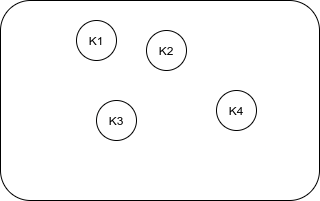
\includegraphics[width=0.7\textwidth]{images/non_det_wallet.png}
	\caption{Nicht-deterministische Wallet\\
	Quelle: Eigene Darstellung}
	\label{6braun:fig:non-deterministic_wallet}
\end{figure}\\
Die fortgeschrittenste Form einer deterministischen ist die sogenannte BIP32-Wallet, welche zwei nützliche Eigenschaften aufweisen kann (BIP steht für \emph{Bitcoin Improvement Proposal} und bezeichnet eine nachträgliche Ergänzung zum Bitcoin-Ökosystem) [\cite{antanopoulos_2014}].
Diese werden in \cite{buterin_2013} als \emph{Master Public Key Property} und \emph{Hierarchy Property} bezeichnet.
Die Master Public Key Property beschreibt die Möglichkeit, aus einem Master Private einen Master Public Key zu generieren, der wiederum alle öffentlichen Schlüssel und deren Adressen erzeugen kann. Dazu berechnet man den sogenannten Offsets, indem man den gewünschten Index und den Master Public Key addiert und das Ergebnis als Input für eine Hashfunktion verwendet. Anschließend addiert man Offset und Master Public Key und erhält den öffentlichen Schlüssel am Index.
$$offset = SHA256(index + masterPubKey)$$
$$pubKey_{index} = offset + masterPubKey$$ Dies geht analog genauso mit dem Master Private Key. 
Aufgrund dieser Eigenschaft ist es möglich, den Master Public Key ungeschützt zu lagern und sogar an dritte Parteien herauszugeben, ohne dass diese Zugriff auf das Guthaben erhalten.\\

Die Hierarchieeigenschaft wird im Kontext einer Organisation mit verschiedenen Organisationszweigen interessant. Ein Geschäftsführer könnte so den unterschiedlichen Geschäftszweigen seines Unternehmens Schlüsselpaare zuweisen, wodurch diese die Verfügungsgewalt über das eigene und Guthaben von Unterstellen erhalten. Gleichzeitig behält der Geschäftsführer die absolute Kontrolle über alle Schlüssel, da er im Besitz der Master Keys ist. Die Abbildung 2.4 zeigt, wie sich eine Organisation die Hierarchieeigenschaft zunutze machen könnte:
\begin{figure}[htpb]
	\centering
	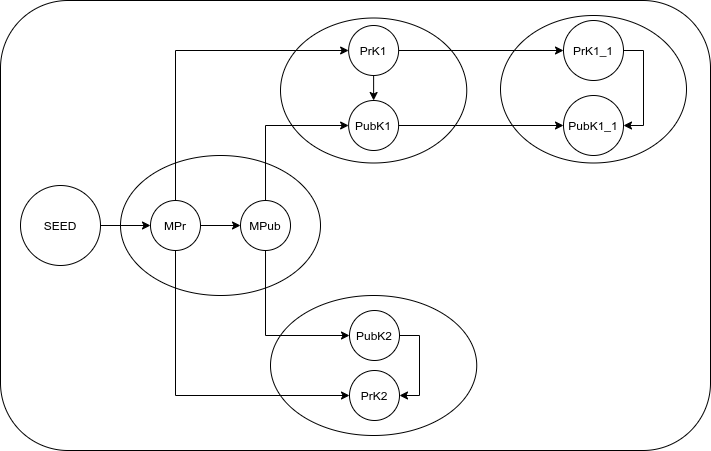
\includegraphics[width=0.7\textwidth]{images/bip32_wallet.png}
	\caption{BIP32-Wallet\\
	Quelle: Eigene Darstellung}
	\label{6braun:fig:_wallet}
\end{figure}
Anders als bei einer nicht-deterministischen Wallet müssen nicht mehr die Private Keys selbst, sondern lediglich der \emph{Seed} gesichert werden. Dieser ist seit dem BIP39/44 eine kurze Liste von für den Menschen leserlichen Worten. Diese können mithilfe eines speziellen Dictionaries in Hex-Zahlen umgewandelt werden, aus denen schließlich der Master Private Key erzeugt wird.
\subsection{Transaktionen}
Damit Bitcoin die Funktion des Zahlungs- bzw. Tauschmittels erfüllen kann, müssen Transaktionen vom Netzwerk ermöglicht werden. In einem \emph{Distributed Ledger}, einer Art dezentraler Datenbank, werden alle Transaktionen im Netzwerk aufgezeichnet. Da es sich um ein gänzlich digitales und dezentrales Netzwerk handelt, sind spezielle Datenstrukturen und Mechanismen nötig.
\subsubsection{Transaction Outputs}
Das Guthaben einer Wallet befindet sich nicht an einem Ort, sondern wird aus \emph{Unspent Transaction Outputs}, kurz UTXO zusammengesetzt, welche alle verfügbaren Gutschriften aus vergangenen Transaktionen darstellen.
Eine Wallet scannt die Blockchain nach allen Outputs, welche mit den Keys des Besitzers assoziiert sind und errechnet damit das gesamte verfügbare Guthaben. Außerdem speichert sie die nötigen Referenzen für den Zugriff auf die UTXO für den späteren Gebrauch in einer Datenbank ab. UTXO sind diskrete, sowie unteilbare Einheiten und können demnach nur in ihrer Gesamtheit genutzt werden. Man betrachte die folgende Abbildung 2.5:
\begin{figure}[htpb]
	\centering
	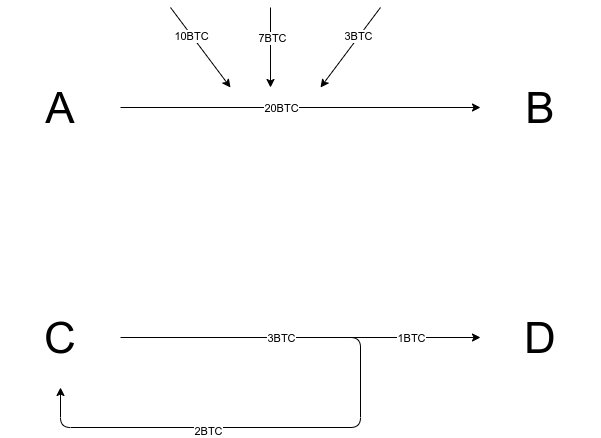
\includegraphics[width=0.7\textwidth]{images/UTXO.png}
	\caption{Transaktionen mit unteilbaren UTXO\\
	Quelle: Eigene Darstellung}
	\label{6braun:fig:Transaktionen}
\end{figure}\\
Für die gewünschte Transaktion von A nach B werden 20 BTC benötigt, die von der Wallet aus verfügbaren UTXO zusammengefügt werden. 
Für das optimale Zusammensammeln von Outputs ist die Wallet zuständig.
C hat für die gewünschte Transaktion von 1 BTC nur 3 BTC zur Verfügung, weshalb diese in ihrer Gesamtheit aufgebraucht werden müssen.
Die übrigen 2 BTC gehen jedoch nicht verloren, sondern landen lediglich wieder als Wechselgeld bei C. 
Die gewünschte Transaktion hat also 2 Outputs.
Jeder Output besteht aus 2 Komponenten: Der Anzahl von BTC und einem sogenannten \emph{Locking Script}, welches nur mithilfe des assoziierten private Keys gelöst werden kann.

\subsubsection{Transaction Inputs}
Das Gegenstück zu den Outputs sind Inputs, über welche die benötigten UTXO für eine Transaktion gesammelt werden. Sie bestehen aus:
\begin{itemize}
	\item Einer ID, über die eine bestimmte Transaktion referenziert wird
	\item Vout, einem Index über den auf bestimmte UTXO der zuvor referenzierten Transaktion zugegriffen wird
	\item Dem Unlocking Script, welches das Locking Script des ausgewählten UTXO löst und mithilfe des privaten Schlüssels erzeugt wird
	\item Einer Sequence, einem optionalen Feld zur Sperrung der Outputs für eine bestimmte Zeit
\end{itemize}
Sowohl Input, als auch Output werden serialisiert und als Byte-Streams im Netzwerk propagiert.\\
\subsubsection{Transaktionskosten}
Abhängig von der Auslastung des Netzwerkes wird eine dadurch bestimmte Menge an Transaktionsgebühren nötig, die sowohl als Anreiz für Bitcoin-Miner, als auch Abschreckungsmechanismus gegen Angriffe durch hochfrequentes Senden von kleinen Transaktionen dienen.
Diese sind zwar kein Muss, jedoch bevorzugen die Miner Transaktionen mit höheren Transaktionskosten. 
Das Berechnen von optimalen Transaktionsgebühren wird normalerweise von der Wallet ausgeführt, jedoch können auch manuelle Transaktionen erstellt werden, die ohne Transaktionskosten langsamer oder gar nicht vom Netzwerk verarbeitet werden.
Bei einer manuellen Transaktion müssen sowohl Inputs, als auch Outputs definiert werden und die Transaktionsgebühren ergeben sich implizit aus der Differenz jener Komponenten. So wie man keine Transaktionsgebühren angegeben kann, ist auch das versehentliche Angeben von zu hohen Gebühren möglich. Man betrachte erneut die Abbildung \ref{6braun:fig:Transaktionen}, in der C 3 BTC an D sendet. Die Transaktion hat 2 Outputs, 1 BTC an D und 2 BTC zurück an C. Sollte der Sender vergessen den 2. Output, welcher das Wechselgeld darstellt, zu definieren, dann werden die gesamten 2 BTC als Transaktionsgebühren für die Transaktion genutzt.
Zusammenfassend lassen sich Transaktionen als Sammlungen von Inputs und Outputs definieren, deren Differenz die genutzten Transaktionskosten darstellen.
\subsection{Die verschiedenen Akteure im Netzwerk}
\cite{nakamoto_whitepaper_2008} nennt das Propagieren von Transaktionen an alle Knoten als ersten Schritt, der zur Instandhaltung des Netzwerkes erforderlich ist. Dieses Kapitel steigt einen Schritt früher ein und befasst sich mit den verschiedenen Akteuren im dezentralen Netzwerk, ihren Rollen sowie den nötigen Schritten zum Eintritt neuer Teilnehmer.
\subsubsection{Rollen}
Trotz fehlender Hierarchien im Netzwerk nehmen die Teilnehmer abhängig von ihren Funktionalitäten verschiedene Rollen ein. Als \emph{Full Node} bezeichnet man Teilnehmer, die alle der folgenden Funktionalitäten erfüllen:
\begin{itemize}
	\item Routing Modul - Kommunikation mit dem Netzwerk
	\item Wallet - Verwaltung von Guthaben
	\item Miner - Finden neuer Blöcke
	\item Full Blockchain - Besitz gesamter Blockchain
\end{itemize}
Diese können selbstständig Transaktionen prüfen, signieren und am Konsens-Algorithmus teilnehmen.\\

Bis auf das Routing-Modul, ohne das die Kommunikation mit dem Netzwerk nicht möglich ist, können sich die Teilnehmer ein Subset der Funktionalitäten heraussuchen und diese erfüllen. 
Beispielsweise benötigt eine Lightweight-Wallet kein Mining und auch keine volle Blockchain. 
Stattdessen lässt sie Transaktionen von einer dritten Partei prüfen und könnte so aufgrund des geringen Speicherbedarfs in einem Internetbrowser laufen.

\subsubsection{Bootstrapping neuen Teilnehmers}
Nach dem Hochfahren muss ein neuer Teilnehmer zunächst mindestens einen anderen im Netzwerk finden. Dabei stehen ihm sogenannte \emph{DNS Seeds} zur Verfügung, die nichts anderes sind als Server, die auf Abfrage Adressen von stabil laufenden Teilnehmern zurückgeben und deren Adressen im Bitcoin-Klienten enthalten sind. 
Alternativ kann ein neuer Knoten auch eine manuelle Verbindung zu einem anderen Teilnehmer eingehen, wenn ihm dessen Adresse bekannt ist.
Sobald ein anderer Teilnehmer gefunden wurde, wird über TCP ein \emph{Handshake} ausgeführt: Der Neue sendet seine Informationen, wie die Version seines Bitcoin-Klienten an den gefundenen Teilnehmer und dieser geht bei Validität der Informationen eine Verbindung mit ihm ein.
Anschließend können sie ihnen bekannte Adressen austauschen, dieser Vorgang wird in Abbildung 2.6 veranschaulicht:
\begin{figure}[htpb]
	\centering
	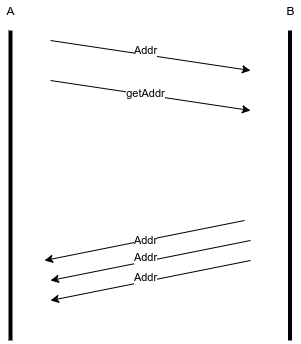
\includegraphics[width=0.5\textwidth]{images/adress_query.png}
	\caption{Teilnehmer tauschen nach erfolgreicher Verbindung Adressen aus\\
	Quelle: vgl. \cite{antanopoulos_2014}}
	\label{6braun:fig:adress_query}
\end{figure}

Ebenso wie sie Adressen miteinander austauschen, werden auch Informationen über den Zustand der Blockchain ausgetauscht. Sollten dem neuen Teilnehmer Blöcke fehlen, versucht er diese von seinen neuen Nachbarn anzufordern, um seine eigene Blockchain zu synchronisieren. Dabei wird der Aufwand auf die verschiedenen Nachbarn aufgeteilt, um einzelne Teilnehmer nicht zu überlasten. Es ist dasselbe Prinzip, wie beim schon länger praktizierten File-Sharing.
\subsection{Blockchain}
Die Blockchain ist die Kerntechnologie des gesamten Protokolls und stellt im Kern eine Datenstruktur mit einer verketteten Liste von Blöcken dar, die wiederum Transaktionen enthalten. 
Die Verkettung erfolgt dadurch, dass jeder Block einen vorher erzeugten referenziert. 
Genauer gesagt enthält der neue Block den SHA256-Hash des Vorgängerblocks, mit dem dieser eindeutig identifizierbar ist. Dadurch wird der Hashwert des Nachfolger verändert und dies wird so für alle folgenden Generationen fortgesetzt. Die folgende Abbildung 2.7 zeigt, wie der zweite Block den Vorgängerblock mithilfe des Hash-Werts referenziert.
\begin{figure}[htpb]
	\centering
	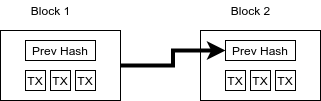
\includegraphics[width=0.5\textwidth]{images/chain.png}
	\caption{Neuer Block referenziert alten Block \\
	Quelle: Eigene Darstellung}
	\label{6braun:fig:chain}
\end{figure}\\

Der daraus entstehende Vorteil ist, dass ein Angreifer bei Veränderung eines vergangenen Blocks die Hashwerte aller Nachfolger neu berechnen muss. Wieso dies mit sehr hohem Rechenaufwand verbunden ist, wird später näher erläutert.

\subsubsection{Datenstruktur}
Die Datenstruktur des Blocks besteht aus mehr Komponenten als dem Vorgänger-Hash und den Transaktionen:
\begin{lstlisting}[mathescape, caption={Datenstruktur des Blocks},captionpos=b]
Block {
	Block Size;
	Block Header;
	Transaction Counter;
	Transactions;
}

Block Header {
	Version;
	Prev Block Hash;
	Merkle Root;
	Timestamp;
	Difficulty Target;
	Nonce;
}
\end{lstlisting}
Der zuvor angesprochene Hashwert wird nicht aus dem gesamten Block, sondern dem \emph{Block Header} errechnet, der Meta-Daten zum Block enthält. Die Komponenten \emph{Merkle Root}, \emph{Difficulty Target} und \emph{Nonce} werden an geeigneter Stelle erläutert.\\

Abgesehen vom Block-Hash lässt sich ein Block auch über die Block-Höhe, was lediglich dem Index des Blocks in der Liste entspricht, identifizieren. 
Dafür folgt man vom Block aus über die Vorgänger der Blockchain, bis man beim sogenannten \emph{Genesis Block}, dem ersten Block, ankommt. 
Anschließend zählt man den Abstand und erhält die Block-Höhe.
Eine eindeutige Identifikation des Blocks ist hierüber allerdings nicht möglich, denn es kann im Falle von \emph{Forks}, die im Kapitel \emph{Der Weg der Transaktion in die Blockchain} erörtert werden, dazu kommen, dass ein Block von mehreren Blöcken als Parent referenziert wird.\\
\subsubsection{Merkle-Tree}
Ein Merkle-Tree ist eine binäre Baumstruktur, bestehend aus den Hashwerten der Transaktionen des Blocks als Blätter. Die Abbildung 2.8 illustriert die Funktionsweise eines Merkle-Trees:
\begin{figure}[htpb]
	\centering
	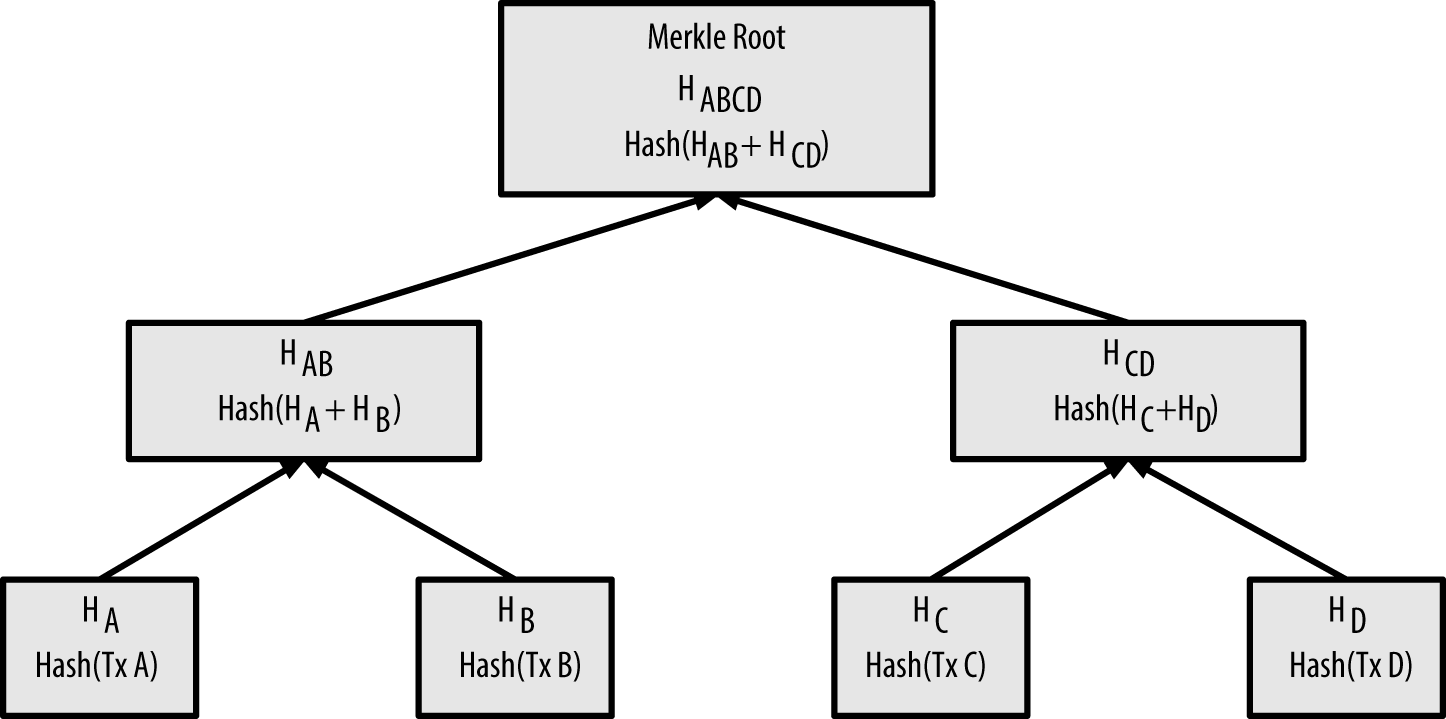
\includegraphics[width=0.7\textwidth]{images/merkle.png}
	\caption{Ein Merkle-Tree\\
	Quelle: \cite{antanopoulos_2014}}
	\label{6braun:fig:merkle}
\end{figure}\\
Auf jeder Ebene werden die Knoten paarweise gehasht, sodass man als Ergebnis die Wurzel als Identität aller Transaktionen im Block erhält. 
Aufgrund einer grundlegenden Eigenschaft von Hash-Funktionen, würde eine minimale Änderung an den Transaktionen die Wurzel, und somit den gesamten Block-Hash völlig verändern. 
Zu beachten ist noch, dass bei einer ungeraden Zahl von Transaktionen die letzte Transaktion in der Liste doppelt im Merkle-Tree aufgeführt wird, um das paarweise Hashing zu ermöglichen.
\subsection{Der Weg der Transaktion in die Blockchain}
Als Folge der dezentralen Struktur des Bitcoin-Netzwerkes ist ein Mechanismus nötig, der Transaktionen ohne ein zentrales Clearinghaus validiert und freigibt. An dieser Stelle kommt das \emph{Mining} ins Spiel, über das zwar neue Bitcoin in Umlauf kommen, aber vor allem ein gemeinsamer Konsens im ganzen Netzwerk erreicht wird.
Dieses Kapitel beschäftigt sich mit den nötigen Schritten für einzelne Transaktionen bis hin zum neuen Block und welche Rolle Miner dabei spielen.
\subsubsection{Miner und ihre Entlohnung}
Miner sind spezielle Teilnehmer im Netzwerk, die darin propagierte Transaktionen aggregieren, validieren und miteinander darum konkurrieren, den nächsten Block zur Blockchain hinzufügen zu dürfen. 
Der Anreiz besteht darin, dass sie für ihren Aufwand, bei erfolgreicher Erweiterung der Blockchain, eine Entlohnung erhalten, die sich aus neuen Bitcoin und gesammelten Transaktionskosten ergibt.\\
Eine Tatsache, mit der Miner leben müssen ist, dass ihre Entlohnung mit der Zeit sinkt. 
Alle 210 000 Blöcke wird die Anzahl neuer Bitcoin halbiert, sodass die Gesamtzahl aller, sich im Umlauf befindenden Bitcoin, gegen 21 Millionen konvergiert. 
Aus diesem Grund wird Bitcoin als \emph{Deflationäre Währung} bezeichnet, die mit der Zeit nicht an Wert verliert, sondern wertvoller wird.
\subsubsection{Sammeln von Transaktionen}
Genau wie alle anderen Teilnehmer sammeln Miner die im Netzwerk propagierten Transaktionen und überprüfen diese. Sollten jene bestimmte Kriterien, wie z.B. eine korrekte Syntax und Korrektheit, nicht erfüllen, werden sie nicht weitergeleitet und verworfen.
Bei Korrektheit sammeln die Teilnehmer validierte Transaktionen in einem Pool und entfernen sie erst dann, wenn ein neuer und valider Block eine der gesammelten Transaktionen beinhaltet. 
Während alle anderen Teilnehmer bei Ankunft eines neuen Blocks lediglich die Transaktionen abgleichen und aus dem Pool entfernen, sammeln Miner übrig gebliebene Transaktionen und starten den Versuch, einen eigenen Block herzustellen.
\subsubsection{Konstruktion des Blocks}
Einen neuen Block zu erstellen ist für Miner aus zwei Gründen attraktiv:
\begin{itemize}
\item Sie erhalten alle Transaktionskosten aus den gesammelten Transaktionen
\item Sie dürfen die sogenannte \emph{Coinbase Transaction} selbst an den Anfang der gelisteten Transaktionen einfügen
\end{itemize}
Das besondere an dieser Transaktion ist, dass sie keine UTXO konsumiert, sondern dem Empfänger neu-generierte Bitcoin ausstellt. Sie augmentiert also nicht das UTXO-Set, sondern erweitert es durch neue Outputs.
Nachdem Miner eine Liste von Transaktionen inklusive Coinbase angelegt haben, konstruieren sie den Block Header bestehend aus Version, Hash des Vorgängerblocks, Wurzel aus dem Merkle-Tree, Zeitstempel, sowie Target und Nonce, die beim Mining eine Rolle spielen, erstellen.
\subsubsection{Mining}
Das Bitcoin-Protokoll ist so konzipiert, dass neue Blöcke in Intervallen von ca. 10 Minuten hinzugefügt werden. 
Um dem Anstieg an Rechenleistung vorzubeugen (man denke an Moore's Law), besitzt das Protokoll die Variable 'Target' als einen eingebauten Schwierigkeitsregler, der je nach Bedarf angepasst werden kann.
Beim Target handelt es sich lediglich um eine Zahl, für die ein darunter liegender Wert durch wiederholtes Hashing des Block Headers, der sich ebenfalls serialisieren lässt, von den Minern gefunden werden muss. 
Falls der Miner keinen geeigneten Hash findet, bedient er sich an der Variable 'Nonce' die als Zählvariable dient und erhöht diese wiederholt, bis es zum Erfolg kommt.
Alle 2016 Blocks wird die gesamte verstrichene Zeit mit der angestrebten Zeit von $2016 * 10 Min$ verglichen und abhängig davon das Target entweder einfacher oder schwerer gemacht. 
Konkret bedeutet dies, den Wert anzupassen, um die Anzahl möglicher darunterliegender Hashwerte entweder zu reduzieren oder vergrößern.
Dieses Verfahren funktioniert, weil ein Hashalgorithmus schon bei einem minimal veränderten Input einen gänzlich anderen Output zurückgibt. 
Gleichzeitig macht es die Fertigung eines Blocks im Voraus unmöglich, da der Hashwert des Vorgängerblocks im neuen Block Header enthalten ist. 
Im wesentlichen besteht das Verfahren also aus dem Konstruieren eines Blocks inklusive Block Header, dessen Hashwert, welcher das Target erfüllt, als 'Proof-of-Work' bezeichnet wird.\\

Während das 'Finden' eines geeigneten Blocks aufwendig ist, müssen andere Teilnehmer den SHA256-Algorithmus nur einmal auf den Block Header anwenden, um den gesamten Block zu validieren. 
Abgesehen vom Hash muss der Block allerdings noch andere Kriterien erfüllen, wie z.B. richtige Zeitstempel oder eine valide Liste von Transaktionen, inklusive valider Coinbase. 
Bei Gutschreibung von zu viel neuen Bitcoin wird der gesamte Block invalide, was betrügerisches Verhalten für Miner unattraktiv macht. Der Block wird nur im Netzwerk propagiert, wenn er die Kriterien erfüllt.\\

Nachdem ein Teilnehmer des Netzwerkes einen neuen Block validiert hat, muss er diesen zu seiner persönlichen Blockchain hinzufügen. Für den neuen Block gibt es drei Szenarios, wie die folgende Abbildung 2.9 zeigt:
\begin{figure}[htpb]
	\centering
	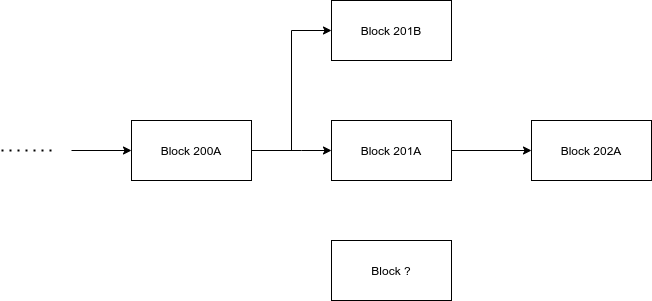
\includegraphics[width=0.7\textwidth]{images/chains.png}
	\caption{Anordnung der Blöcke in einer Kette\\
	Quelle: Eigene Darstellung}
	\label{6braun:fig:chains}
\end{figure}\\
Das erste Szenario ist das Erweitern der Mainchain, also der längsten Kette, und ist dann der Fall, wenn der neue Block (hier 202A) den Kopf dieser als Eltern-Block referenziert.
Die zweite Möglichkeit besteht darin, dass der neue Block an einem inneren Block ansetzt und es dadurch zu einer Verzweigung, also einer neuen Sidechain kommt (hier 201B). Auch wenn dies im ersten Moment unnötig wirkt, werden die Sidechains angesammelt und bei jedem neuen Block mit der Mainchain verglichen, sodass sie, falls mehr Blöcke in diesen enthalten sind, zur neuen Mainchain werden.
Die dritte und letzte Möglichkeit für neue Blöcke (abgesehen von invaliden Blöcken, die verworfen werden) sind sogenannte \emph{Orphans}, also verwaiste Blöcke. Diese referenzieren einen Eltern-Block, der unbekannt ist, weshalb sie bis zur Veröffentlichung dessen in einem Pool gehalten werden. Dies kann dann der Fall sein, wenn Eltern- und Kind-Block in kurzer Zeit hintereinander gefunden werden und als Folge dessen bei manchen Teilnehmern in umgekehrter Reihenfolge ankommen. Auch wenn es in Folge des Minings zu Verzweigungen kommt, finden die Teilnehmer im Netzwerk immer einen gemeinsamen Konsens, indem sie der längsten Validen Kette, die am meisten Proof-of-Work 'angesammelt' hat, folgen. Miner konzentrieren sich dann darauf, für diese Kette neue Blöcke zu finden.\\

Wenn zwei Miner, die man auch als Kontrahenten in einem Wettkampf sehen kann, in relativ kurzer Zeit jeweils einen neuen Block finden, kann es zu einem sogenannten \emph{Fork} kommen. Beide propagieren ihren gefundenen Block als neuen Kopf der längsten Chain und nehmen den Block des Gegners in einer Sidechain auf. Abhängig davon, welchen Block sie zuerst erhalten, folgen die anderen Teilnehmer dem Sender des ersten Blocks und geben ihm ihr Stimmrecht. Selbst bei einer gleichmäßigen Verteilung des Stimmrechts findet sich nach weiteren Generationen schließlich die Wahre Mainchain, da das gleichzeitigen Blöcken relativ selten ist.
Eine zweite Möglichkeit für Forks sind sogenannte \emph{Hard Forks}, bei denen man eine Sidechain in dem Wissen weiterführt, dass sie nie zur Mainchain wird. Dies kann beispielsweise der Fall sein, wenn eine Gruppe von Teilnehmern nicht mit der Funktionsweise des Protokolls zufrieden sind und eine erweiterte Blockgröße fordern, um mehr Transaktionen zuzulassen. Man schreibt also ein neues Protokoll, welches eine Sidechain fortführt und von den daran interessierten Nutzern genutzt wird. Dies war der Hintergrund zur Entstehung von \emph{Bitcoin Cash}.
\subsection{Angriff auf das Netzwerk}
Um einen bösartigen Angriff auf das dezentrale System ausüben zu können, muss man 51\% der dem Netzwerk zur Verfügung stehenden Rechenleistung besitzen. Ist dieser Umstand gegeben, haben Angreifer folgende Optionen:
\begin{itemize}
	\item Es kann ein 'Double Spending' ausführt werden
	\item Einzelnen Teilnehmern kann die Anteilnahme am Netzwerk untersagt werden
\end{itemize}
Unter normalen Umständen ist Double Spending nicht möglich, doch Angreifer könnten Bitcoin auf eine Handelsbörse überweisen und dort in einer gewünschte Währung auszahlen lassen. Anschließend setzen sie mit einer Sidechain dort an, wo sich das Guthaben noch beim Angreifer befindet, also die UTXO ungenutzt sind, und erweitern diese zur neuen Mainchain.
Die zweite Möglichkeit des Angriffs besteht darin, dass einzelne Teilnehmer von der Anteilnahme ausgeschlossen werden, indem man beispielsweise ihre Transaktionen nicht in neue Blöcke aufnimmt. Das Gleiche gilt für bestimmte Miner, deren Blöcke man gezielt ablehnen kann.\\

Aufgrund der immensen Rechenleistung, die dafür nötig wäre, wird ein Angriff in tieferen Schichten teurer und wäre, abgesehen von durch Konzerne oder Staaten finanzierten Attacken, unwahrscheinlich.